\chapter{Materiales, Métodos e Implementación}

\section{Materiales}
Para la realización de este TFM se dispone de una colección de 497 modelos 3D de la sínfisis del pubis, correspondientes tanto al lado izquierdo como derecho, en formato de malla OBJ. Estos modelos fueron escaneados por el personal del Laboratorio de Antropología Física del Departamento de Medicina Legal, Toxicología y Antropología Física de la Universidad de Granada. Además de la digitalización tridimensional, el equipo del laboratorio examinó cuidadosamente cada una de las muestras y etiquetó manualmente los atributos correspondientes a las características morfológicas observables en la superficie de la sínfisis del pubis así como la edad real de fallecimiento de los individuos, datos que también han sido provistos dentro de un fichero de Microsoft Excel.

\begin{figure}[h]
    \centering
    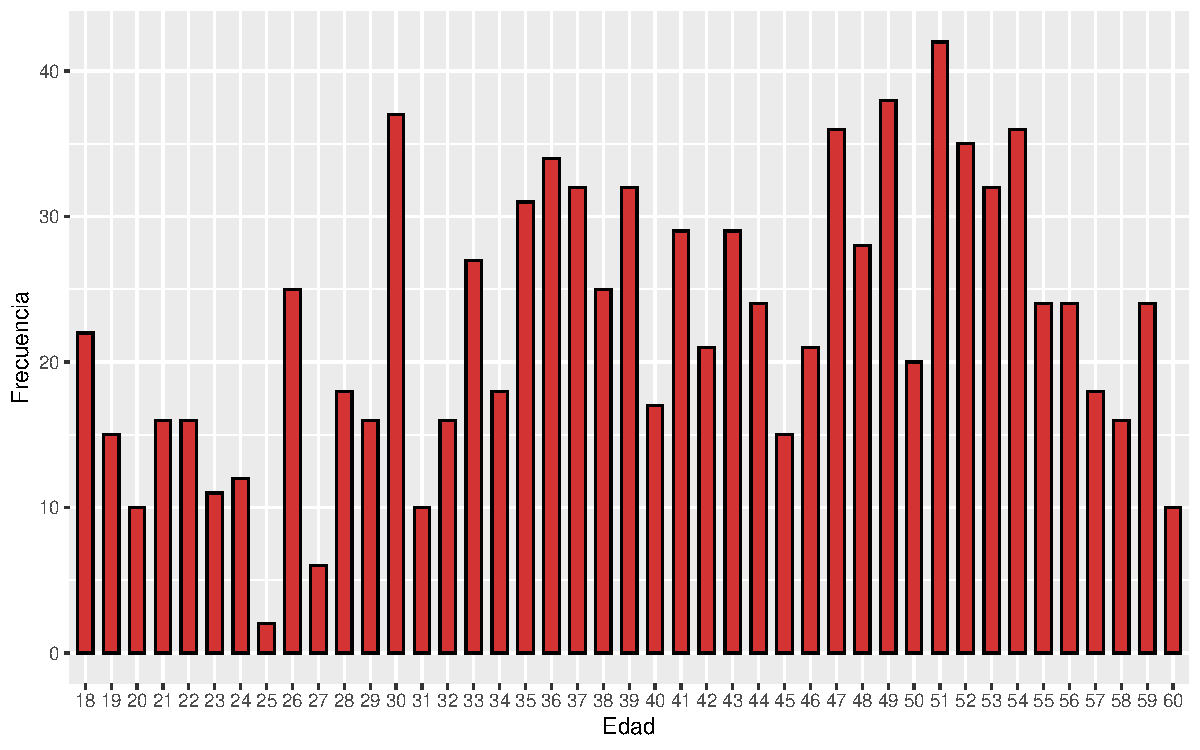
\includegraphics[width=\linewidth]{../../scripts/eda/eda_univar/char_age_distr.pdf}
    \caption[Distribución de los datos por edad]{Distribución de los datos las edades conocidas de los sujetos}
    \label{fig4:age}
\end{figure}
\begin{figure}[h]
    \centering
    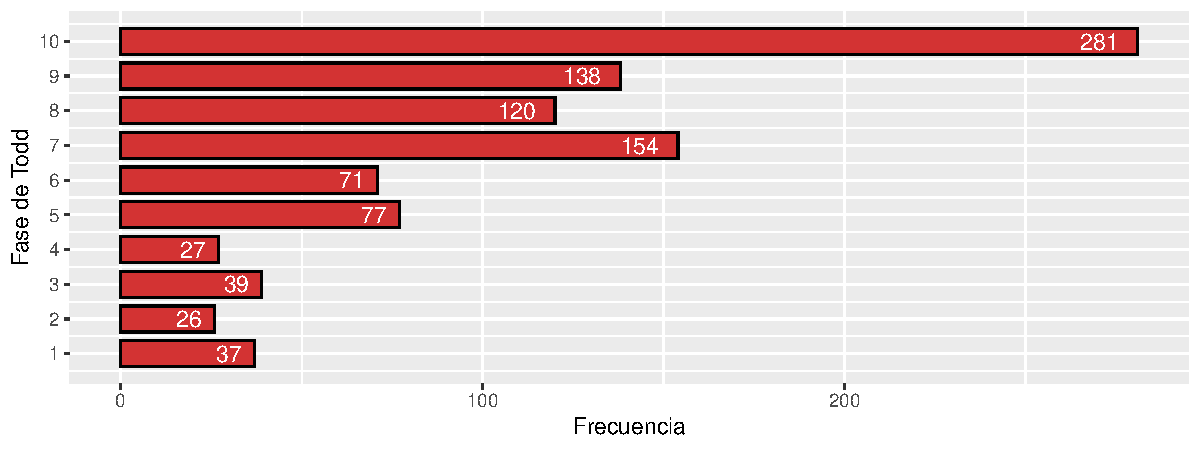
\includegraphics[width=\linewidth]{../../scripts/eda/eda_univar/char_t_phase_distr.pdf}
    \caption[Distribución de los datos por cada rango de edad]{Distribución de los datos por cada rango de edad del método de Todd. \textbf{1}: 18-19 años, \textbf{2}: 20-21 años, \textbf{3}: 22-24 años, \textbf{4}: 25-26 años, \textbf{5}: 27-30 años, \textbf{6}: 30-35 años, \textbf{7}: 35-39 años, \textbf{8}: 39-44 años, \textbf{9}: 45-50 años, \textbf{10}: 50+ años.}
    \label{fig4:todd_phase}
\end{figure}

\subsection{Análisis Exploratorio de Datos}
Realizando un análisis exploratorio de los datos (\textit{Exploratory Data Analisys}, EDA), se observa que la muestra está compuesta por individuos de entre 18 y 60 años, como se muestra en la Figura \ref{fig4:age}. Además, estos individuos han sido clasificados dentro de las 10 fases del método de Todd, tal como se aprecia en la Figura \ref{fig4:todd_phase}.

De ambos gráficos se aprecia que las edades más representadas corresponden a individuos de mayor edad, lo cual es coherente considerando el origen de los datos. Sin embargo, este patrón también evidencia un desbalance inherente en la muestra, un fenómeno esperado cuando se trabaja con datos reales.

\subsubsection{Análisis Univariable}
Continuando con el EDA enfocado en las nueve características del método de Todd, se observa un claro desbalance en la distribución de clases, como se muestra en las gráficas correspondientes en la Figura \ref{fig4:todd_chars}. Las clases más representadas son coherentes con las manifestaciones morfológicas que el hueso de la sínfisis del pubis presenta a edades más avanzadas.

Desde la perspectiva del balance de datos, las características de Borde Dorsal (Subfigura \ref{fig4:todd_chars__use}), Nódulo Óseo (Subfigura \ref{fig4:todd_chars__bn}), Plataforma Dorsal (Subfigura \ref{fig4:todd_chars__dp}) y Borde Inferior (Subfigura \ref{fig4:todd_chars__lse}) presentan un desbalance particularmente acentuado, con aproximadamente 95\%, 91\%, 90\% y 90\% de las muestras concentradas en una sola clase, respectivamente. Este fuerte desbalance sugiere que estas características podrían tener un rendimiento limitado al ser utilizadas para el entrenamiento de modelos de DL.

El resto de las características muestra un desbalance menos extremo, con entre el 60\% y el 70\% de los datos agrupados en una única clase. La característica con mayor equilibrio en su distribución es el Bisel Ventral (Subfigura \ref{fig4:todd_chars__vb}), en la que los datos se reparten aproximadamente en un 33\% por clase, dado que esta posee tres clases distintas. Se espera que esta característica, junto con aquellas que presenten menos desbalance, proveerán mejores resultados al ser entrenadas por la red.

\subsubsection{Correlaciones}

\begin{figure}
    \centering
    \begin{subfigure}{\textwidth}
        \centering
        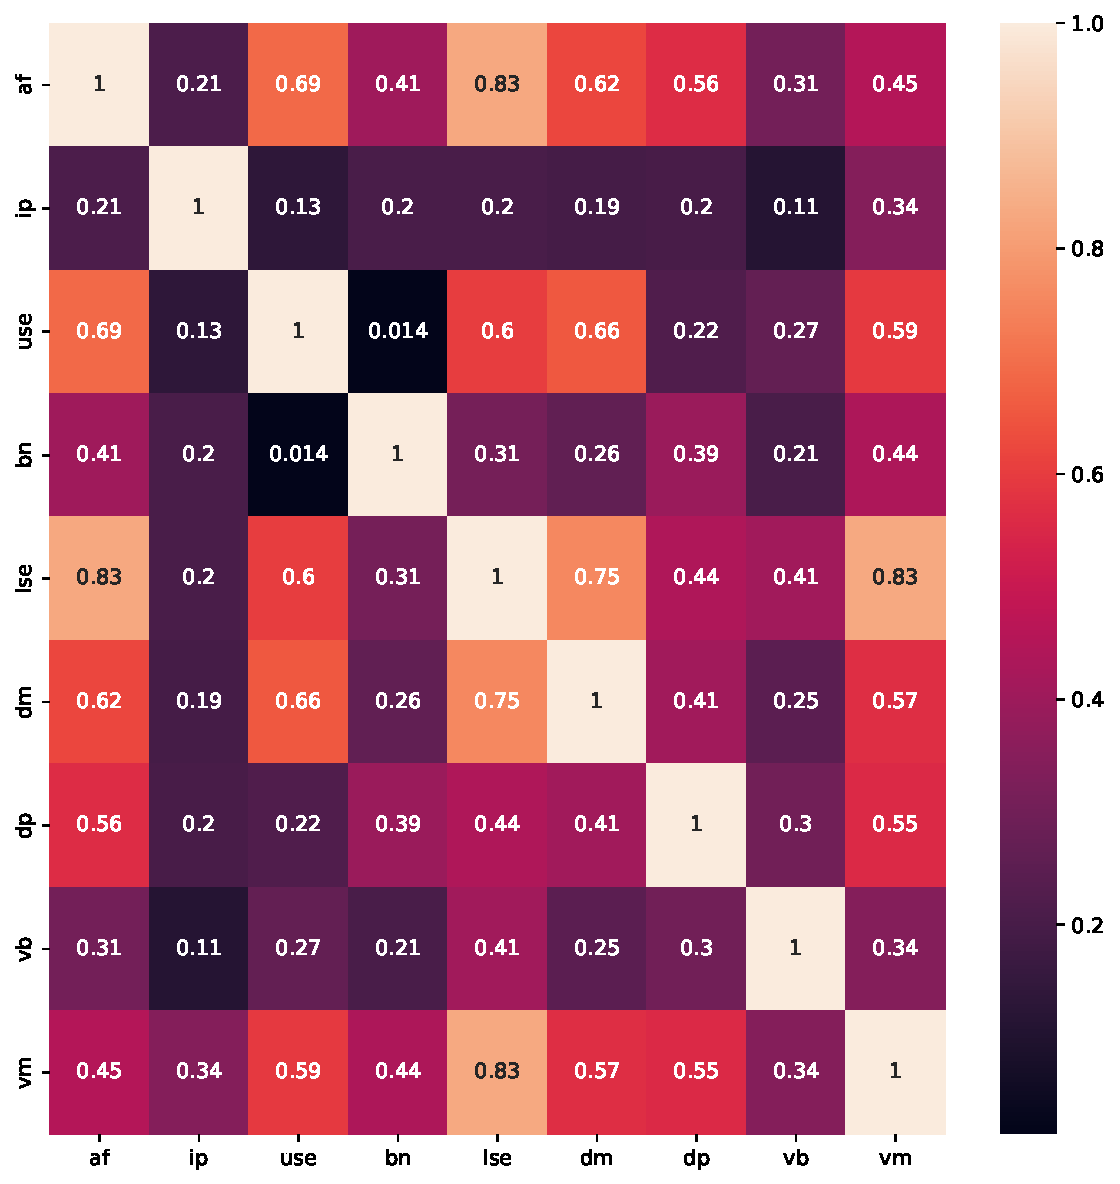
\includegraphics[width=0.7\linewidth]{../../scripts/eda/assoc_plot_cramersv.pdf}
        \caption{Correlograma usando la V de Cramér}
        \label{fig4:todd_chars__cramersv}
    \end{subfigure}
    \begin{subfigure}{\textwidth}
        \centering
        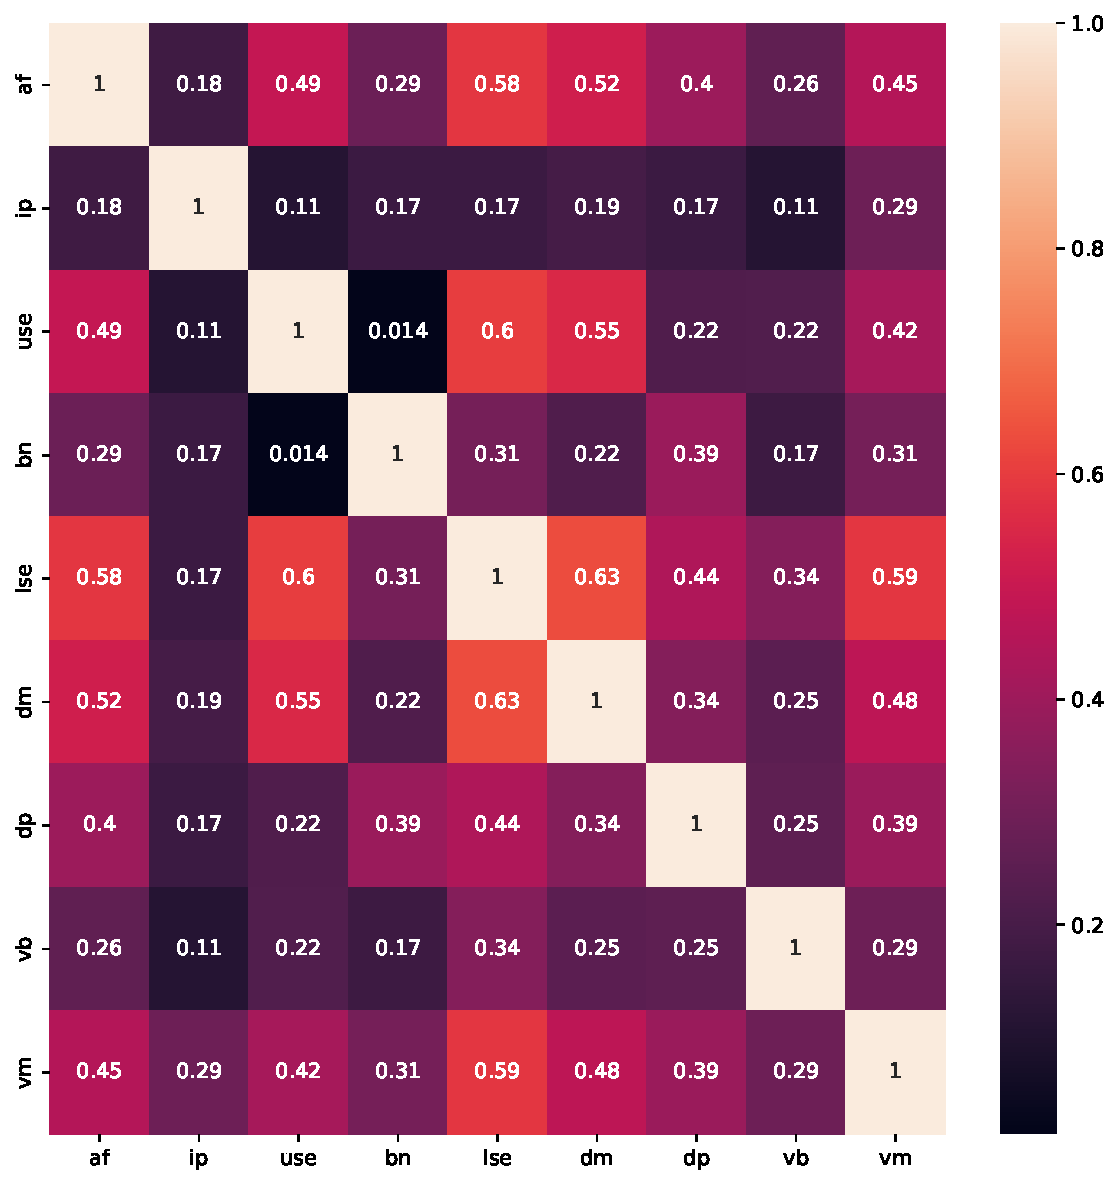
\includegraphics[width=0.7\linewidth]{../../scripts/eda/assoc_plot_tschuprow.pdf}
        \caption{Correlograma usando la T de Tschuprow}
        \label{fig4:todd_chars__tschuprow}
    \end{subfigure}
    \caption[Correlogramas entre características de Todd]{Correlogramas entre las características de Todd}
    \label{fig4:todd_chars_correlogram}
\end{figure}

Si bien los datos empleados en este estudio no son de naturaleza tabular y se utilizan técnicas de DL que no requieren una extracción manual de características, resulta igualmente útil de cara a los experimentos analizar las correlaciones existentes entre las nueve características de Todd. Dado que dichas variables son categóricas, se ha optado por utilizar la V de Cramér, una medida estadística que cuantifica el grado de asociación entre dos variables categóricas. Además, para corregir el sesgo que puede surgir al trabajar con tablas de contingencia no cuadradas, se ha complementado el análisis con la T de Tschuprow, la cual atenúa dicho efecto y permite una interpretación más equilibrada de la asociación entre las variables.

Ambos correlogramas se presentan en la Figura \ref{fig4:todd_chars_correlogram}, donde puede apreciarse que las correlaciones entre las características de Todd varían significativamente entre sí. Como era de esperarse, existen discrepancias entre los valores obtenidos mediante la V de Cramér y la T de Tschuprow, siendo esta última más conservadora en presencia de tablas de contingencia no cuadradas. Para facilitar la interpretación de estos resultados, se ha incluido la Tabla \ref{table4:corr}, en la que se listan las tres características con mayor correlación para cada una.

Del análisis se concluye que las características LSE, AF y VM son, en general, las que presentan los mayores niveles de correlación con el resto, lo que sugiere una mayor dependencia entre ellas. En contraste, la característica IP muestra los niveles más bajos de correlación con las demás, seguida de BN, lo cual puede indicar un comportamiento más independiente. Este conocimiento será especialmente relevante en los experimentos de entrenamiento en modo multietiqueta, ya que incorporar características correlacionadas entre sí podría favorecer el aprendizaje del modelo y mejorar su rendimiento.

\begin{table}[h]
    \centering
    \begin{tabular}{|c|cc|}
    \hline
    \rowcolor[HTML]{D33333} 
    \cellcolor[HTML]{D33333}{\color[HTML]{FFFFFF} } & \multicolumn{2}{c|}{\cellcolor[HTML]{D33333}{\color[HTML]{FFFFFF} Características con mayor asociación}} \\ \cline{2-3} 
    \rowcolor[HTML]{D33333} 
    \multirow{-2}{*}{\cellcolor[HTML]{D33333}{\color[HTML]{FFFFFF} Característica}} & \multicolumn{1}{c|}{\cellcolor[HTML]{D33333}{\color[HTML]{FFFFFF} V de Cramér}} & {\color[HTML]{FFFFFF} T de Tschuprow} \\ \hline
    AF & \multicolumn{1}{c|}{LSE, USE, DM} & LSE, DM, USE \\
    BN & \multicolumn{1}{c|}{\textbf{VM, AF, DP}} & \textbf{DP, LSE, VM} \\
    DM & \multicolumn{1}{c|}{LSE, USE, AF} & LSE, USE, AF \\
    DP & \multicolumn{1}{c|}{\textbf{AF, VM, LSE}} & \textbf{LSE, AF, BN} \\
    IP & \multicolumn{1}{c|}{\textbf{VM, AF, LSE}} & \textbf{VM, DM, AF} \\
    LSE & \multicolumn{1}{c|}{\textbf{VM, AF, DM}} & \textbf{DM, USE, VM} \\
    USE & \multicolumn{1}{c|}{AF, DM, LSE} & LSE, DM, AF \\
    VB & \multicolumn{1}{c|}{LSE, VM, AF} & LSE, VM, AF \\
    VM & \multicolumn{1}{c|}{\textbf{LSE, USE, DM}} & \textbf{LSE, DM, AF} \\ \hline
    \end{tabular}
    \caption{Cuadro resumen de las correlaciones más fuertes entre cada característica de Todd}
    \label{table4:corr}
\end{table}

\begin{figure}[h]
    \centering
    \begin{subfigure}{\textwidth}
        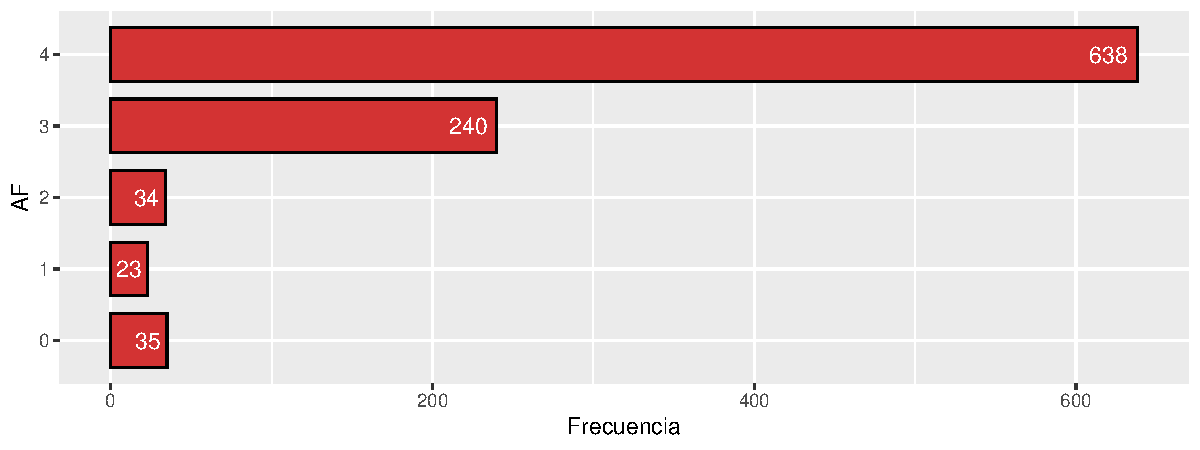
\includegraphics[width=\linewidth]{../../scripts/eda/eda_univar/char_af_distr.pdf}
        \caption{Crestas y Surcos (\textit{Auricular Face}, AF)}
        \label{fig4:todd_chars__af}
    \end{subfigure}

    \begin{subfigure}{\textwidth}
        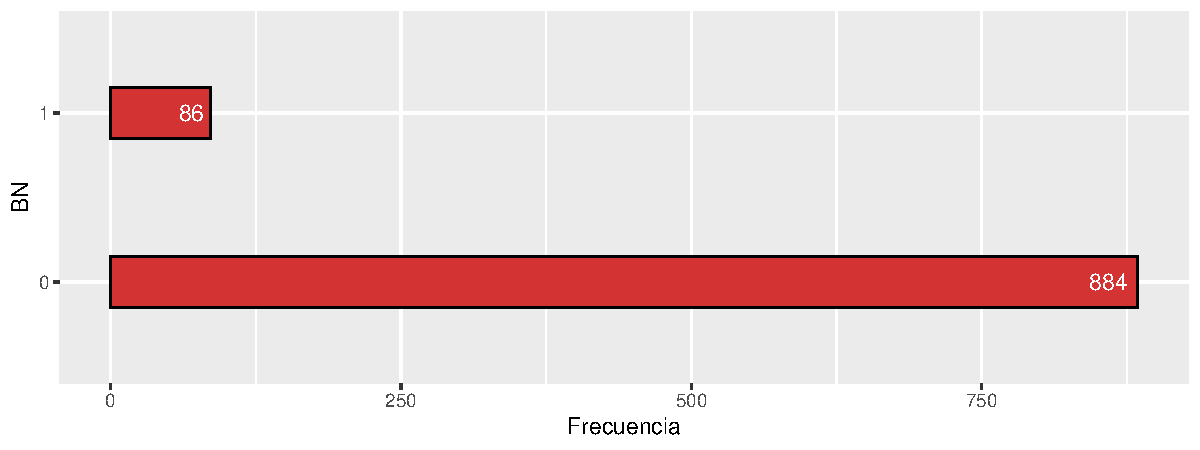
\includegraphics[width=\linewidth]{../../scripts/eda/eda_univar/char_bn_distr.pdf}
        \caption{Nódulo Óseo (\textit{Bony Nodule}, BN)}
        \label{fig4:todd_chars__bn}
    \end{subfigure}
    
    \begin{subfigure}{\textwidth}
        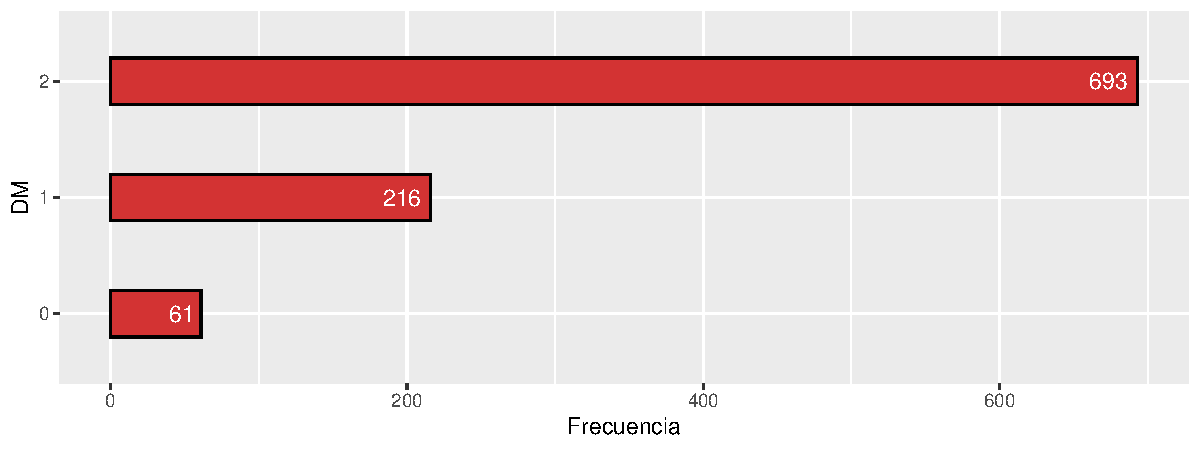
\includegraphics[width=\linewidth]{../../scripts/eda/eda_univar/char_dm_distr.pdf}
        \caption{Borde Dorsal (\textit{Dorsal Margin}, DM)}
        \label{fig4:todd_chars__dm}
    \end{subfigure}
    \phantomcaption

\end{figure}
\begin{figure}
    \ContinuedFloat

    \begin{subfigure}{\textwidth}
        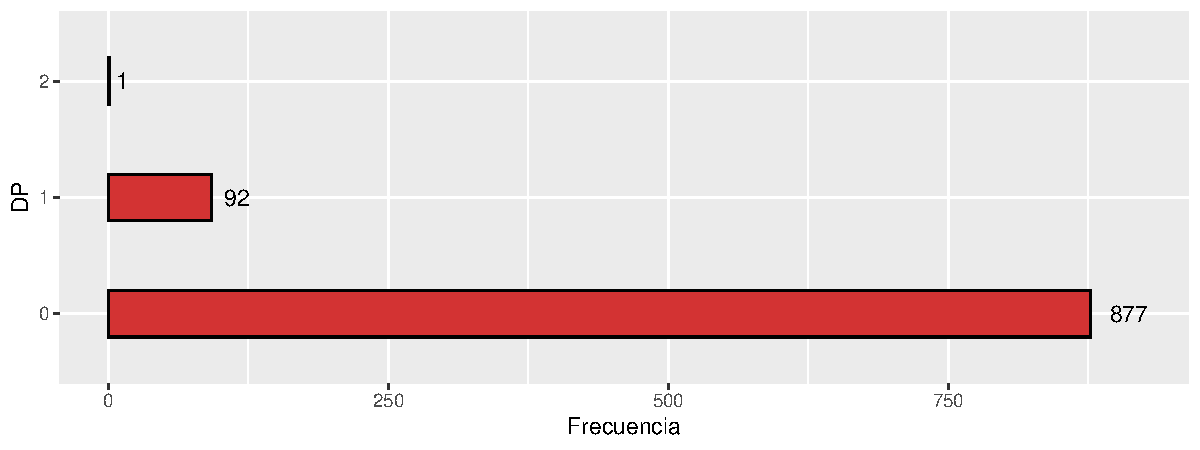
\includegraphics[width=\linewidth]{../../scripts/eda/eda_univar/char_dp_distr.pdf}
        \caption{Plataforma Dorsal (\textit{Dorsal Plateau}, DP)}
        \label{fig4:todd_chars__dp}
    \end{subfigure}

    \begin{subfigure}{\textwidth}
        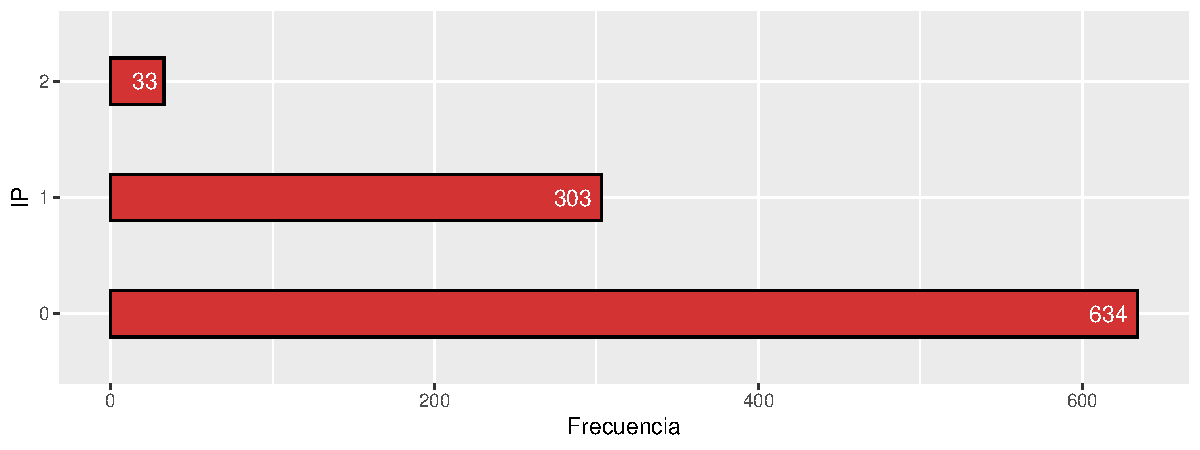
\includegraphics[width=\linewidth]{../../scripts/eda/eda_univar/char_ip_distr.pdf}
        \caption{Porosidad Irregular (\textit{Irregular Porosity}, IP)}
        \label{fig4:todd_chars__ip}
    \end{subfigure}

    \begin{subfigure}{\textwidth}
        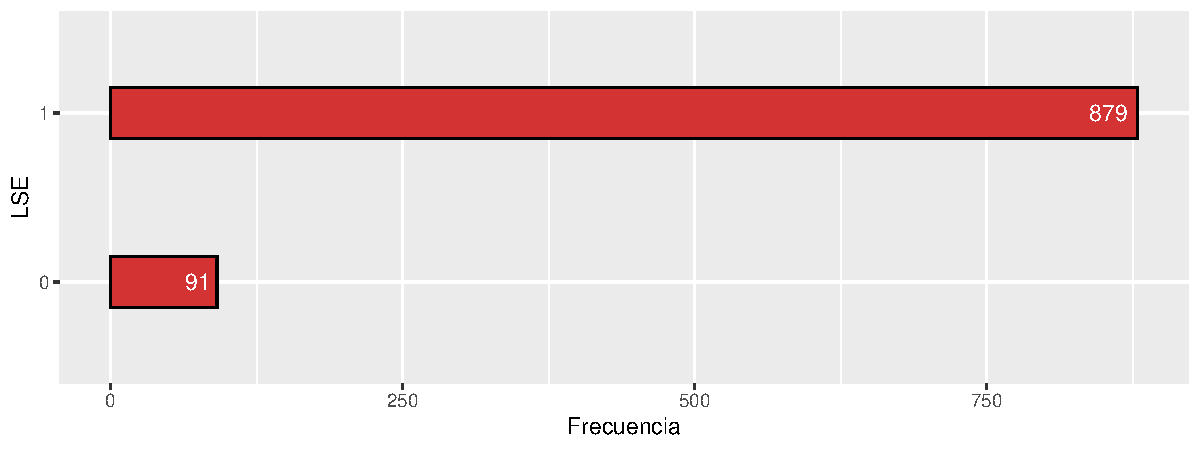
\includegraphics[width=\linewidth]{../../scripts/eda/eda_univar/char_lse_distr.pdf}
        \caption{Borde Inferior (\textit{Lower Symphysial Extremity}, LSE)}
        \label{fig4:todd_chars__lse}
    \end{subfigure}

    \phantomcaption
    \label{fig4:todd_chars}
\end{figure}
\begin{figure}
    \ContinuedFloat

    \begin{subfigure}{\textwidth}
        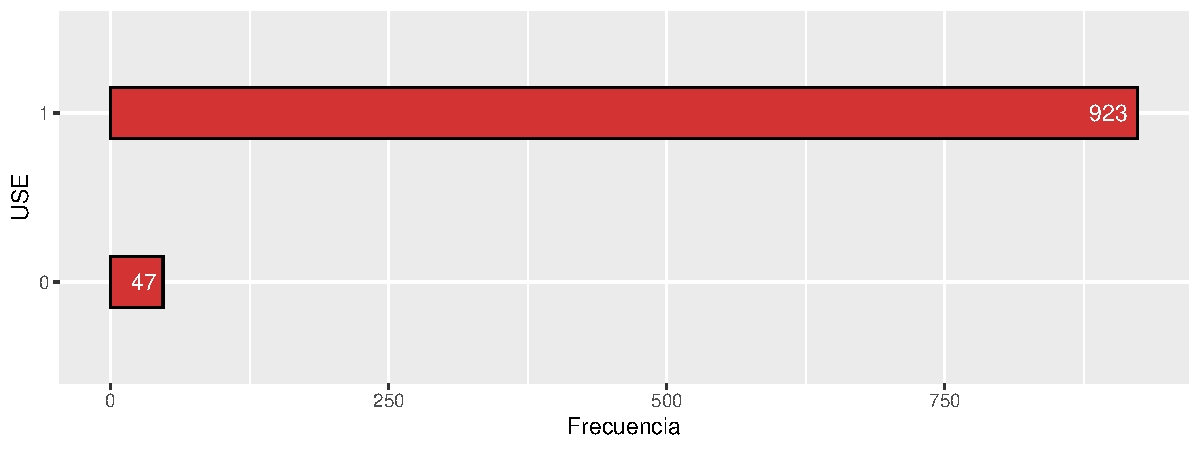
\includegraphics[width=\linewidth]{../../scripts/eda/eda_univar/char_use_distr.pdf}
        \caption{Borde Dorsal (\textit{Upper Symphysial Extremity}, USE)}
        \label{fig4:todd_chars__use}
    \end{subfigure}

    \begin{subfigure}{\textwidth}
        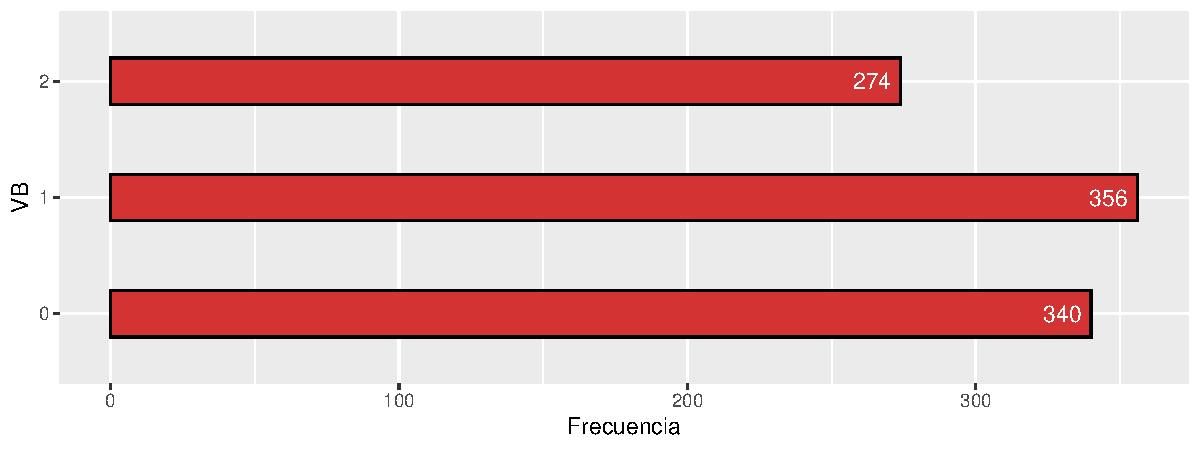
\includegraphics[width=\linewidth]{../../scripts/eda/eda_univar/char_vb_distr.pdf}
        \caption{Bisel Ventral (\textit{Ventral Bevel}, VB)}
        \label{fig4:todd_chars__vb}
    \end{subfigure}

    \begin{subfigure}{\textwidth}
        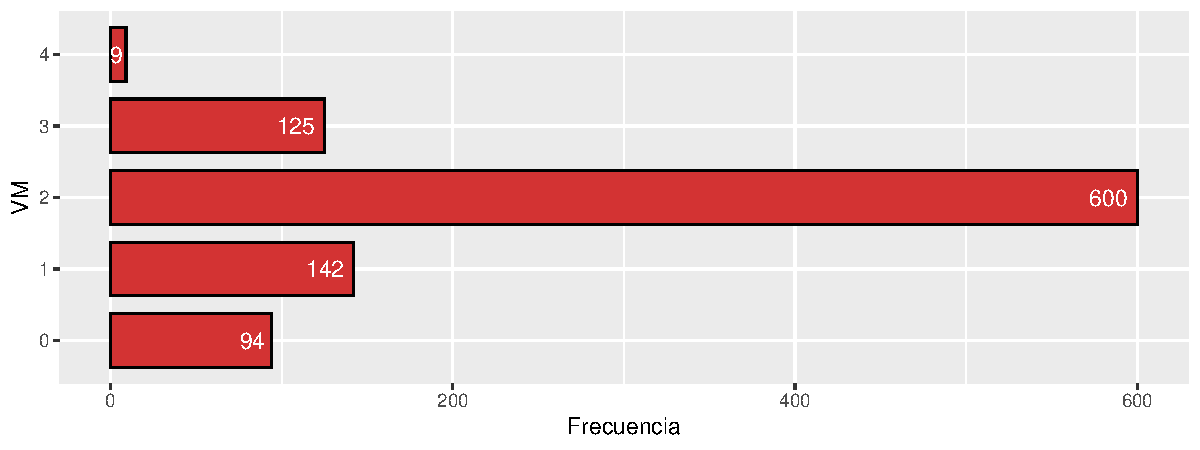
\includegraphics[width=\linewidth]{../../scripts/eda/eda_univar/char_vm_distr.pdf}
        \caption{Borde Ventral (\textit{Ventral Margin}, VM)}
        \label{fig4:todd_chars__vm}
    \end{subfigure}
    \caption[Distribución de las características de Todd]{Distribución de las características de Todd en los datos}

\end{figure}

\subsubsection{Preparación de los datos}
De la muestra original de 497 individuos, es decir, un total de 986 huesos correspondientes a las sínfisis del pubis izquierda y derecha, fue necesario eliminar 16 muestras por diversos motivos: presencia de deformidades anatómicas, ausencia del archivo OBJ asociado o falta de correspondencia entre el modelo 3D y los datos etiquetados provistos. Se opta por utilizar las 970 muestras restantes en su totalidad, ya que en problemas de DL es fundamental contar con un volumen de datos considerable, aunque estos estén altamente desbalanceados, pues se pueden utilizar diversas técnicas para mitigar el efecto que produce esto al rendimiento de un modelo. 

Cabe destacar que, en el caso de la característica Plataforma Dorsal (Subfigura \ref{fig4:todd_chars__dp}), la clase 3 (\say{Presente}) cuenta con solo una muestra, lo cual impide que el modelo pueda aprender representaciones significativas para dicha clase. Por tanto, esta muestra será eliminada durante el entrenamiento de modelos de DL que hagan uso de dicha característica. Además, la Clase 2 originalmente denominada \say{En Formación} será renombrada a \say{Presente}, con el objetivo de mantener la consistencia semántica.

Las 970 mallas presentan una resolución media de 994,601 triángulos, con un mínimo de 329,438 y un máximo de 1,688,348 triángulos. Para poder aplicar el método ExMeshCNN, descrito en la Sección \ref{section4:methods}, es necesario que todas las mallas tengan una resolución uniforme. Una opción inicial considerada fue remuestrear las mallas al número medio de triángulos; sin embargo, este tamaño resulta inviable computacionalmente con el hardware disponible.

Por esta razón, se ha procedido a reducir la resolución de las mallas a 100,000, 50,000 y 25,000 triángulos, empleando las técnicas detalladas en la Sección \ref{???}. Tal como se demuestra en los experimentos descritos en la Sección \ref{???}, esta reducción no compromete significativamente la fidelidad de la superficie original. La variación entre las superficies del modelo original y las versiones reducidas es mínima, lo que permite afirmar que las mallas simplificadas conservan en mayor o menor grado parte de la información morfológica relevante para los experimentos.

Adicionalmente, el método requiere que las mallas no contengan geometría degenerada y que estén completamente selladas (es decir, que no exista geometría \textit{non-manifold} y que sea \textit{watertight}, según la terminología en gráficos por ordenador). Dado que estas mallas provienen de escaneos de objetos anatómicos reales, es esperable que algunas presenten incompletitud o defectos estructurales, lo que impide su uso directo con ExMeshCNN. Para solventar estos problemas, se aplicaron técnicas de reparación y sellado descritas en la Sección \ref{???}, con el objetivo de restaurar la geometría y garantizar la integridad topológica de cada modelo antes de ser procesado por la red neuronal.

\section{Métodos}
\label{section4:methods}
Como se ha mencionado previamente en la Sección \ref{section3:meshes}, ExMeshCNN \cite{kim_exmeshcnn_2022} representa el estado del arte en el procesamiento de mallas poligonales mediante redes neuronales profundas. A continuación, se detalla cómo este \textit{framework} adapta el concepto de convolución para que pueda aplicarse de manera efectiva sobre datos tridimensionales.



\section{Implementación}
\label{section4:implementation}